% it/figures/data_pipeline/fig_anomalies.tex — versione italiana
\begin{figure}[!ht]
    \centering
    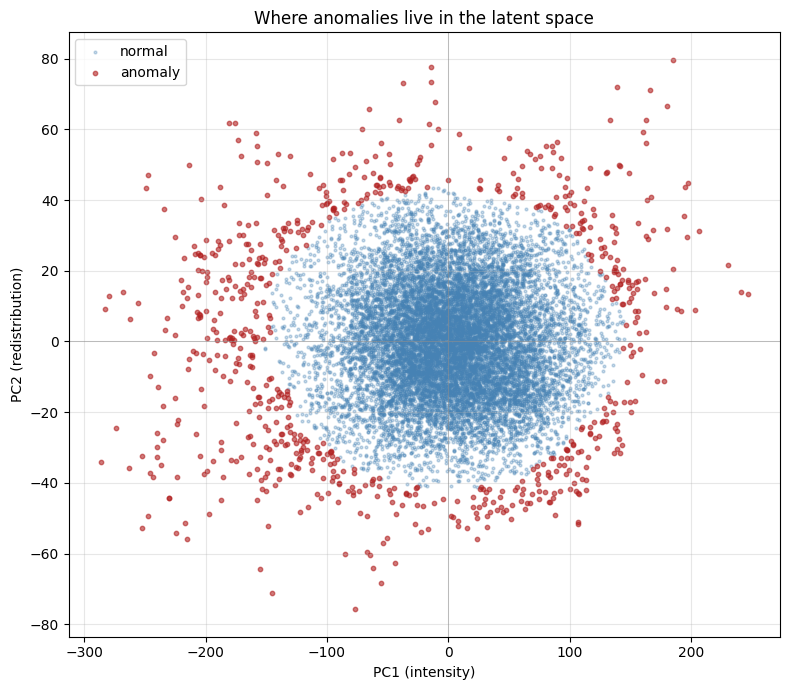
\includegraphics[width=0.9\textwidth]{figures/data_pipeline/anomalies.png}
    \caption[Anomalie Isolation Forest lungo il record.]{\textbf{Eventi anomali
    discreti, distribuiti lungo il record.} L'Isolation Forest segnala il
    \SI{5}{\percent} dei profili (730) come anomali nel piano PC1--PC2. Si addensano
    nel 2009--2010 (158 profili), nel 2012--2013 (100) e nel 2018 (66), senza trend nel
    tempo --- a conferma del risultato nullo di preallarme da un metodo diverso. Questi
    momenti diventano texture percepibile (principio di grammatica~P3) nel
    Capitolo~\ref{ch:translate}.}
    \label{fig:anomalies}
\end{figure}
